\documentclass[10pt]{article}
\usepackage[margin=0.8in]{geometry}
\usepackage{amsmath,amssymb,amsthm,mathtools,bm}
\usepackage{graphicx}
\usepackage{booktabs}
\usepackage{enumitem}
\usepackage{microtype}
\usepackage{caption}
\usepackage{titlesec}
\usepackage[colorlinks=true,linkcolor=black,citecolor=black,urlcolor=black]{hyperref}

\titlespacing*{\section}{0pt}{1.1ex}{0.5ex}
\titlespacing*{\subsection}{0pt}{0.9ex}{0.4ex}
\titleformat{\section}{\normalfont\large\bfseries}{\thesection.}{0.6em}{}
\titleformat{\subsection}{\normalfont\normalsize\bfseries}{\thesubsection}{0.6em}{}
\setlist[itemize]{leftmargin=1.3em,topsep=1pt,itemsep=1pt,parsep=0pt}
\setlist[enumerate]{leftmargin=1.5em,topsep=1pt,itemsep=1pt,parsep=0pt}
\setlength{\parskip}{1pt}
\setlength{\abovedisplayskip}{2.5pt}
\setlength{\belowdisplayskip}{2.5pt}
\setlength{\abovedisplayshortskip}{1.5pt}
\setlength{\belowdisplayshortskip}{1.5pt}
\captionsetup{font=small,labelfont=bf,skip=2pt}
\graphicspath{{figures/}{slides/figures/}}

\newtheorem{proposition}{Proposition}
\newtheorem{corollary}{Corollary}
\newtheorem{conjecture}{Conjecture}

\newcommand{\R}{\mathbb{R}}
\newcommand{\T}{^{\!\top}}
\newcommand{\op}{\mathrm{op}}
\newcommand{\eff}{\mathrm{eff}}
\newcommand{\pair}{\mathrm{pair}}
\newcommand{\stat}{\mathrm{stat}}
\newcommand{\Gw}{\widetilde{G}}
\newcommand{\Mw}{\widetilde{M}}
\newcommand{\fit}{\mathrm{fit}}
\DeclareMathOperator{\Cov}{Cov}
\DeclareMathOperator{\Corr}{Corr}
\DeclareMathOperator{\CV}{CV}
\DeclareMathOperator{\tr}{tr}
\DeclareMathOperator{\diag}{diag}

\title{\vspace{-2.2em}\Large\bfseries When Does Raw AGOP Explain Learned Features?\\[-0.2em]\normalsize A Weighted Stationarity View of Two-Layer Feature Learning}
\author{Angelo Farfan}
\date{\vspace{-1.0em}\small Final Project Report\vspace{-1.4em}}

\begin{document}
\maketitle

\begin{abstract}\noindent\small
The Neural Feature Ansatz (NFA) observes that a trained network's first-layer feature matrix tracks an average gradient outer product (AGOP). We ask what the optimization itself implies in a two-layer model with square loss and $L_2$ regularization on the first layer. Expanding the first-layer stationarity equation gives an exact, finite-sample answer: the stable convergence-side object is not raw AGOP but a \emph{residual-weighted} AGOP, $H^2 \approx \kappa_{\eff}\,\Gw$, and $\Gw$ is exactly the covariance of the input gradients of the loss. Raw AGOP is then a derived, regime-dependent shadow of this law, gated by two checkable links: a scalar \emph{beta bridge} and \emph{high-gain pair closure}. The weighted-law error is an exact sum of a pushed pair-isotropy term and a stationarity defect, and we show the pushed term is what matters: a large global pair defect can coexist with a tiny pushed error. We classify how each link fails, prove the two links are logically independent, and report a synthetic-network study: across nine teacher-student families and five seeds, the weighted law is empirically robust, even to constructions built to break high-gain pair closure, and degrades only under persistent-residual outlier structure, which also bends the beta link.
\end{abstract}

\section{Introduction}

The NFA, posited by Radhakrishnan et al.~\cite{radhakrishnan2024mechanism} and central to recursive feature machines, states that the learned first-layer geometry $H := B\T B$ of a trained network is proportional to a power of the AGOP $G := \tfrac{1}{n}\sum_i \nabla f(x_i)\nabla f(x_i)\T$. Empirically the relation is striking, but a general nonlinear theory is open: for deep networks, NFA-type statements have been proved only in linear regimes, with nonlinear counterexamples~\cite{tansley2025nfa}. The Features-at-Convergence viewpoint (FACT)~\cite{boixadsera2025fact} reframes the question, deriving a self-consistent feature relation from first-order optimality rather than fitting AGOP after training, and explaining when NFA holds or fails.

This report takes that viewpoint literally in the simplest nonlinear model that has the structure: a two-layer network trained with square loss and ridge on the first layer. Expanding the first-layer stationarity equation gives a clean answer with three pieces. \textbf{(1) The natural object is residual-weighted, not raw}: stationarity yields a deterministic identity $H^2 - \kappa_{\eff}\Gw = (\lambda^2 n^2)^{-1} B\T(S - d_{\eff}T)B + B\T E_{\stat}B$, where $\Gw$ is the residual-weighted AGOP, which equals the covariance of the input gradients of the loss, so the convergence-side object is derived rather than assumed. \textbf{(2) Raw AGOP needs two extra links}: a scalar \emph{beta bridge} ($\Mw \approx \beta M$) converts $\Gw$ into $G$, and the weighted law itself requires \emph{high-gain pair closure}. We give exact identities for both and the failure taxonomy they imply, and a $2$-dimensional argument shows the two links are logically independent, so no theorem with hypotheses limited to stationarity and finite-dimensional algebra can imply a universal raw NFA law. \textbf{(3) The right pair diagnostic is not the global one}: the pushed pair error $B\T(S - d_{\eff}T)B$ factors through a stationarity-induced gain map, so a large global pair-isotropy defect can be conservative. The contribution is this finite-sample decomposition, the diagnostics that read those links off any checkpoint, and a synthetic study mapping which link fails where. Closely related concurrent work studies $B\T B$ as a feature-dynamics object via a ``Virtual Covariance''~\cite{cha2026virtual}, and feature-learning \emph{dynamics} in two-layer networks from small initialization is studied separately~\cite{kunin2025agf}.

\section{Setup and first-order identities}

The model is $f(x) = a\T \phi(Bx)$ with $B \in \R^{m\times d}$, $a \in \R^m$, smooth activation $\phi$. With training data $(x_i,y_i)_{i=1}^n$, residuals $r_i := f(x_i)-y_i$, and hidden-derivative features $q_i := a \odot \phi'(Bx_i)$, write $X = [x_1,\dots,x_n]$, $Q = [q_1,\dots,q_n]$, $R = \diag(r_1,\dots,r_n)$. By the chain rule $\nabla f(x_i) = B\T q_i$. Define
\[
M := \tfrac{1}{n}QQ\T, \qquad \Mw := \tfrac{1}{n}QR^2Q\T, \qquad G := B\T M B, \qquad \Gw := B\T \Mw B = \tfrac{1}{n}\sum_i r_i^2 \nabla f(x_i)\nabla f(x_i)\T.
\]
Since the per-sample loss is $\ell_i = \tfrac12 r_i^2$ and $\nabla_x \ell_i = r_i \nabla f(x_i)$, the weighted object is exactly the covariance of the input gradients of the loss: $\Gw = \tfrac1n \sum_i \nabla_x\ell_i\,\nabla_x\ell_i\T$. Training minimizes $\mathcal L(B,a) = \tfrac{1}{2n}\sum_i r_i^2 + \tfrac{\lambda}{2}\|B\|_F^2$, so $\nabla_B \mathcal L = \tfrac{1}{n}QRX\T + \lambda B$, and at exact $B$-stationarity
\[
B = -\tfrac{1}{\lambda n}QRX\T, \qquad\text{with defect}\qquad Z := \lambda n B + QRX\T.
\]
The residual weighting is not a modeling choice. It is the derivative of the square loss, and it enters $B$ automatically.

\section{The deterministic weighted square law}

Let $T := QR^2Q\T = n\Mw$, $S := QRX\T X RQ\T$, $d_{\eff} := \langle S,T\rangle_F / \|T\|_F^2$ (the best Frobenius scalar fitting $S \approx dT$), and $\kappa_{\eff} := d_{\eff}/(\lambda^2 n)$. From $\lambda n B = -QRX\T + Z$ we get $BB\T = (\lambda^2 n^2)^{-1}S + E_{\stat}$ with $E_{\stat} := (\lambda^2 n^2)^{-1}(-QRX\T Z\T - ZXRQ\T + ZZ\T)$. Multiplying by $B\T(\cdot)B$ and using $H^2 = B\T(BB\T)B$ gives the central result.

\begin{proposition}[Deterministic weighted law]\label{prop:weighted}
With the notation above,
\[
H^2 - \kappa_{\eff}\Gw = \tfrac{1}{\lambda^2 n^2}\,B\T(S - d_{\eff}T)B + B\T E_{\stat}B,
\qquad\text{hence}\qquad
\|H^2 - \kappa_{\eff}\Gw\|_\op \le \|B\|_\op^2\!\left(\tfrac{\|T\|_\op}{\lambda^2 n^2}\,\mathcal A_{\pair} + \|E_{\stat}\|_\op\right),
\]
where $\mathcal A_{\pair} := \big\|T^{\dagger/2}(S - d_{\eff}T)T^{\dagger/2}\big\|_\op$. In particular, if $Z=0$ and $S = d_{\eff}T$ on $\mathrm{range}(T)$, then $H^2 = \kappa_{\eff}\Gw$ exactly.
\end{proposition}

\paragraph{The pushed pair error is the operative quantity.} The bound uses $\mathcal A_{\pair}$, the worst pair-isotropy error over the whole support of $T$, but the law only sees the term $B\T(S - d_{\eff}T)B$. Let $QR = U\Sigma V\T$ be the thin SVD ($U\in\R^{m\times r}$ in hidden space, $V\in\R^{n\times r}$ in sample space), and set $H_X := V\T X\T X V$, $F_X := H_X - d_{\eff}I_r$, $G_{\stat} := \Sigma^2 V\T X\T$. Then $S - d_{\eff}T = U\Sigma F_X \Sigma U\T$, $\mathcal A_{\pair} = \|F_X\|_\op$, and at exact stationarity, since $B = -(\lambda n)^{-1}U\Sigma V\T X\T$,
\[
B\T(S - d_{\eff}T)B = \tfrac{1}{\lambda^2 n^2}\,G_{\stat}\T F_X\,G_{\stat}.
\]
So $F_X$ is the pair-isotropy defect of the input geometry $X\T X$ \emph{restricted to the sample combinations the residual-weighted hidden gradients use}, $G_{\stat}$ weights each such direction by $\sigma_k^2$ and projects it through $X\T$, and the weighted law breaks only when $F_X$ is large on the high-gain directions of $G_{\stat}$. A large global $\mathcal A_{\pair} = \|F_X\|_\op$ with all the defect on low-gain directions costs almost nothing. A sufficient probabilistic mechanism: if a high-gain right-singular subspace $W = V P_{\mathrm{hi}}$ is fixed or independent of Gaussian $X$, then $W\T X\T X W \approx dI$ by standard Wishart concentration, so $F_X$ is small there. The catch is that the learned $W$ depends on $X$, so this is a sufficient condition, not a proof for trained networks (Sec.~\ref{sec:exp}). Upgrading it requires an adaptive-concentration argument over a low-complexity class of learnable subspaces.

\section{From weighted to raw AGOP, and the failure taxonomy}

Raw AGOP needs a scalar bridge $\Mw \approx \beta M$. The Frobenius best-fit one is $\beta_{\fit} := \langle \Mw, M\rangle_F / \|M\|_F^2$. Using $\langle q_iq_i\T, q_jq_j\T\rangle_F = (q_i\T q_j)^2$,
\[
\beta_{\fit} = \frac{\sum_{i,j} r_i^2 (q_i\T q_j)^2}{\sum_{i,j}(q_i\T q_j)^2} = \frac{1}{n}\sum_i \ell_i\, r_i^2, \qquad \ell_i := \frac{\sum_j (q_i\T q_j)^2}{\tfrac1n\sum_k\sum_j(q_k\T q_j)^2}, \quad \tfrac1n\sum_i \ell_i = 1,
\]
i.e.\ $\beta_{\fit}$ is a hidden-gradient-leverage-weighted average of the squared residuals, with $\min_i r_i^2 \le \beta_{\fit} \le \max_i r_i^2$. Hence
\[
\frac{\beta_{\fit}}{\bar r^2} - 1 = \Corr_n(\ell, r^2)\,\CV_n(\ell)\,\CV_n(r^2), \qquad \bar r^2 := \tfrac1n\sum_i r_i^2,
\]
so the beta bridge tracks mean residual energy precisely when hidden-gradient leverage and residual energy are weakly correlated. Combining with Prop.~\ref{prop:weighted}: if $\|H^2 - \kappa_{\eff}\Gw\|_\op \le E_w$ and $\|\Gw - \beta_{\fit}G\|_\op \le E_\beta$, then $\|H^2 - \kappa_{\eff}\beta_{\fit}G\|_\op \le E_w + \kappa_{\eff}E_\beta$, and solving for $G$ divides by $|\beta_{\fit}|$. So the raw conversion is well conditioned only away from interpolation, where $\beta_{\fit}$ is bounded away from zero. This is the \emph{two-regime picture}: $H^2 \approx \kappa_{\eff}\Gw$ is the stable late object, while $H^2 \approx \kappa_{\eff}\beta_{\fit}G$ (raw-AGOP-like) is visible only in an intermediate regime.

\paragraph{Failure taxonomy.} Three distinct mechanisms break NFA-type behavior. \emph{(i) Beta failure}: $\Corr_n(\ell,r^2)$ is large, so $\beta_{\fit}$ deviates from $\bar r^2$, the raw law is biased, but the weighted law is unaffected. \emph{(ii) High-gain pair failure}: $F_X$ is large on the high-gain directions of $G_{\stat}$, so $G_{\stat}\T F_X G_{\stat}$ is large and the weighted law itself fails. \emph{(iii) Late-regime collapse}: near interpolation $\beta_{\fit}\to 0$, so the raw conversion is ill-conditioned even when the weighted law is exact. A fourth case is benign: $\mathcal A_{\pair}$ large but the pushed error small (the conservative-diagnostic case). The two links are logically independent: there are explicit $2$-dimensional stationary instances ($n=2$, $\lambda n = 1$) where (a) the weighted law is exact while $\Mw = \beta M$ has no scalar solution, (b) the beta bridge is exact while a high-gain pair defect breaks the weighted law, and (c) $\mathcal A_{\pair}$ is order one while the pushed error is $O(\varepsilon^2)$. Consequently:

\begin{corollary}\label{cor:no-universal}
No theorem whose only hypotheses are exact $B$-stationarity and finite-dimensional algebra can imply a universal exact raw scalar NFA law $H \approx cG^\alpha$. The two bridge conditions (beta stability and high-gain pair closure) are required.
\end{corollary}

\section{Experiments}\label{sec:exp}

\paragraph{Protocol.} All data are synthetic teacher-student regression. For each run, a fixed random two-layer teacher $f_*(x) = a_*\T \phi(B_* x)$ labels $n=128$ inputs $x_i \in \R^{256}$ drawn from a chosen distribution (clean labels), and a fresh two-layer student ($m=16$ hidden units) is trained on those pairs with square loss plus ridge on $B$ ($\lambda = 10^{-2}$), using gradient descent followed by L-BFGS refinement, in double precision, logging the diagnostics at roughly $170$ checkpoints. We run five random seeds per family. At each checkpoint we evaluate exactly the objects of Prop.~\ref{prop:weighted} and Sec.~4: the weighted residual $\|H^2 - \kappa_{\eff}\Gw\|_\op$, the theorem bound, $\beta_{\fit}/\bar r^2$ and $\Corr_n(\ell,r^2)$, the global $\mathcal A_{\pair}$ versus the pushed pair error $\|B\T(S - d_{\eff}T)B\|_\op/(\lambda^2 n^2)$, and the stationarity defect. Quantities are read at the best-stationarity checkpoint (smallest $\|BB\T - B_{\stat}B_{\stat}\T\|_\op$) unless noted. The data families are three positive controls (isotropic Gaussian, anisotropic Gaussian, low-rank signal plus isotropic noise) and six adversarial families built to attack a specific link (rare hard and rare easy high-leverage clusters, two-region gating, mixture of subspaces, strongly anisotropic Gaussian, and a low-rank signal with a steeply anisotropic within-subspace covariance).

\begin{figure}[t]
\centering
\begin{minipage}[t]{0.40\textwidth}\centering
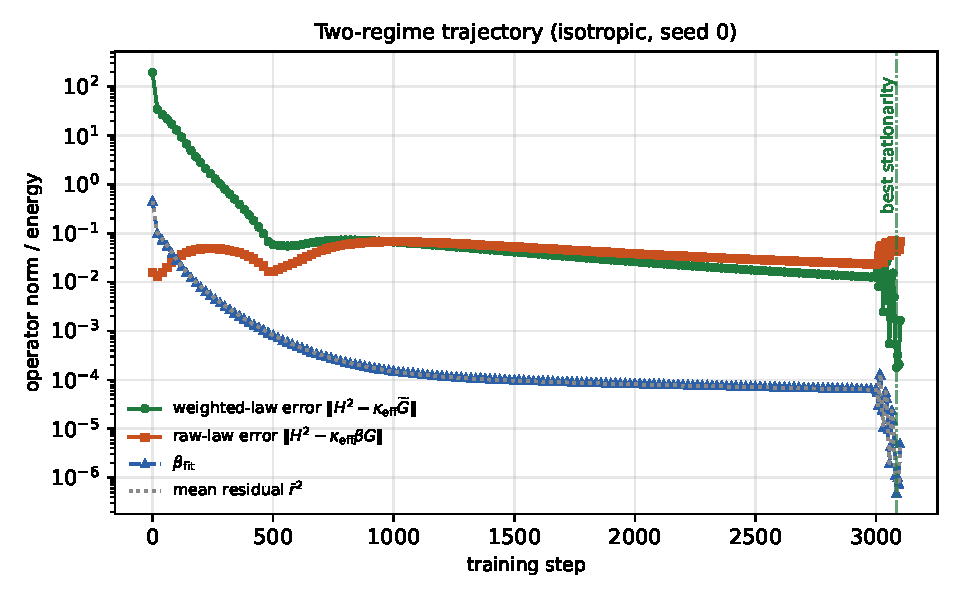
\includegraphics[width=\linewidth]{two_regime_isotropic_seed_0.pdf}
\caption{Two-regime trajectory (isotropic, one seed). Green: weighted-law error. Red: raw-AGOP error. Blue: $\beta_{\fit}$. The weighted-law error decreases into stationarity, the raw error bottoms out in an intermediate window, and $\beta_{\fit}$ collapses with the mean residual energy near interpolation ($\min_i r_i^2 \le \beta_{\fit} \le \max_i r_i^2$). The step at the gradient-descent-to-L-BFGS hand-off is a real regime change, not a plotting artifact.}
\label{fig:traj}
\end{minipage}\hfill
\begin{minipage}[t]{0.55\textwidth}\centering
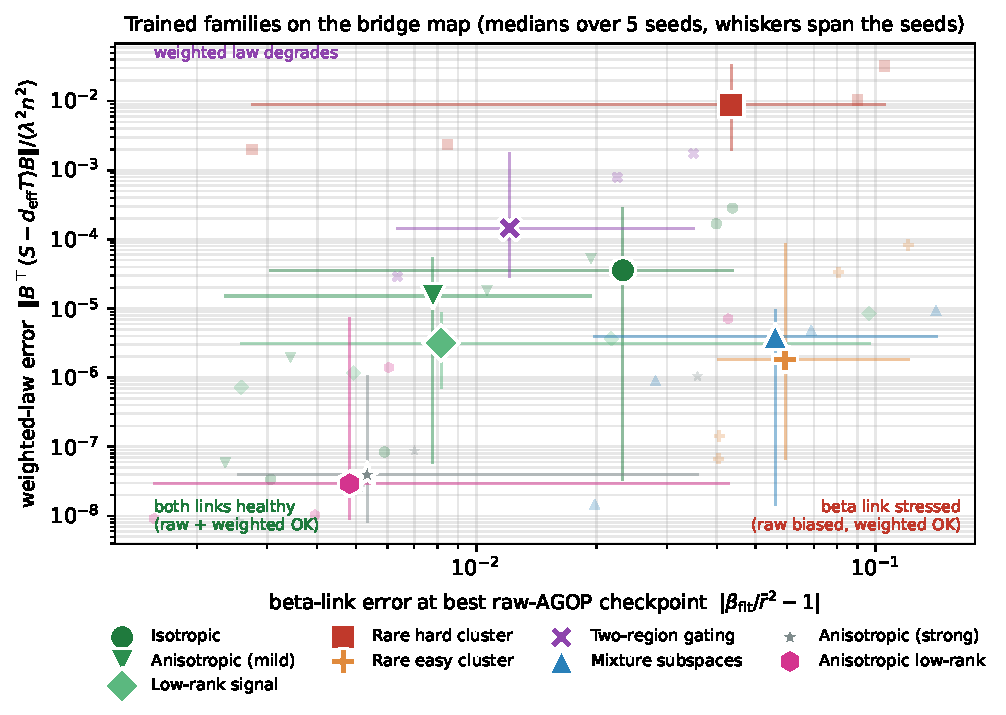
\includegraphics[width=\linewidth]{phase_diagram.pdf}
\caption{Trained families on the bridge map (5 seeds, markers at family medians, whiskers span the seeds). $x$: beta-link error $|\beta_{\fit}/\bar r^2 - 1|$ at the best raw-AGOP checkpoint. $y$: weighted-law residual $\|B\T(S - d_{\eff}T)B\|/(\lambda^2 n^2)$ at the best-stationarity checkpoint. The positive families and the two pair-geometry attacks (strong anisotropy, anisotropic low-rank) sit in the bottom-left healthy cluster. The mixture and rare-easy families move right (beta link stressed, weighted law fine), and only the rare hard cluster moves up by orders of magnitude (two-region gating, mildly).}
\label{fig:phase}
\end{minipage}
\end{figure}

\paragraph{Positive families.} At best-stationarity checkpoints the weighted law is accurate and within its deterministic bound: mean weighted residual $\approx 3.6\times10^{-3}$, $1.9\times10^{-3}$, $6.4\times10^{-4}$ for the isotropic, anisotropic, and low-rank-signal families, with mean theorem-bound ratios $\approx 0.15$, $0.090$, $0.099$. The beta bridge is benign: $\beta_{\fit}/\bar r^2$ averages $0.99$, $1.00$, $1.02$ across seeds, with small spread. And the global pair diagnostic is conservative: $\mathcal A_{\pair}$ averages roughly $80$ to $280$ while the pushed pair error averages $\approx 5.6\times10^{-5}$, $1.1\times10^{-5}$, $2.5\times10^{-6}$, five to seven orders of magnitude smaller, exactly the case the SVD factorization predicts. Figure~\ref{fig:traj} shows the trajectory: a single end-of-training correlation number hides the structure that the decomposition makes explicit.

\paragraph{Trained bridge map and a robustness finding.} Figure~\ref{fig:phase} places all nine families on axes given by the two links. The headline observation is that the weighted law is hard to break. Two families built deliberately to attack high-gain pair closure, a strongly anisotropic Gaussian (covariance spectrum spanning four orders of magnitude) and a low-rank signal with a steeply anisotropic within-subspace covariance, both land in the healthy bottom-left cluster with the positive controls, with pushed pair errors near $10^{-7}$ even though their global $\mathcal A_{\pair}$ and even their high-gain closure norms are sizeable. The reason is structural: near stationarity $B = -(\lambda n)^{-1}QRX\T$, so the only directions that enter the pushed error are the ones the residual-weighted hidden gradients span, and the network self-aligns those directions with the input geometry, keeping $S \approx d_{\eff}T$ on exactly the directions $B$ sees. The mixture-of-subspaces and rare-easy families instead move right: they stress the beta link ($|\beta_{\fit}/\bar r^2 - 1|$ rises to about $0.05$, raw AGOP biased), while the weighted law stays fine. The only family that moves up by orders of magnitude is the rare hard cluster (and, mildly, two-region gating): there, amplified outlier labels keep the residuals of a small set large persistently, sustaining a misaligned $QR$ that the network cannot iron out at stationarity, and that same persistence also bends the beta link, so it is a combined failure rather than a pure pair one. In these runs the weighted law degrades only under persistent-residual outlier structure.

\section{Discussion}

\paragraph{Relation to recent work.} AGOP and recursive feature machines~\cite{radhakrishnan2024mechanism} make AGOP a central object of feature learning, and FACT~\cite{boixadsera2025fact} derives convergence-side feature relations from first-order optimality and explains when NFA holds. The present work is the concrete two-layer square-loss specialization of that mechanism, with the novel part being the bridge decomposition: identifying $\Gw$ as the loss-gradient covariance, isolating the beta and high-gain-pair links, showing the global pair diagnostic is conservative, and mapping which link fails where. Deep-NFA theory proves NFA in linear regimes with nonlinear counterexamples~\cite{tansley2025nfa}, consistent with Corollary~\ref{cor:no-universal}. Concurrent work studies $B\T B$ as a feature-dynamics object via a Virtual Covariance and a Feature Learning Equation~\cite{cha2026virtual}, and relating that quantity to $\Gw$ is a natural next step. Feature-learning dynamics from small initialization is treated by alternating gradient flows~\cite{kunin2025agf}, a candidate tool for the open dynamics direction below.

\paragraph{Limitations.} The model is two-layer with square loss and ridge on $B$ only, and the families are synthetic. The deterministic identity assumes exact stationarity. We report near it and log $E_{\stat}$ so its contribution is visible, and the theorem bound uses the conservative $\mathcal A_{\pair}$, so the bound ratio is well below one rather than tight. The high-gain pair-closure result is conditional (a frozen-subspace concentration mechanism), not a proof for trained networks. The trained map is a guiding map across nine families, not a deliberate grid sweep over the leverage-residual correlation crossed with high-gain anisotropy, and per-seed spread is wide while family medians separate cleanly.

\paragraph{Open directions.} (i) Derive the beta decorrelation (or high-gain pair closure) from training dynamics rather than assuming it. The relevant empirical probe, whether high hidden-gradient leverage predicts faster residual decay, is logged. (ii) Isolate a pure high-gain pair failure: every pair-geometry attack so far self-aligns near stationarity. (iii) A full deliberate phase diagram with samplewise diagnostics, and one non-synthetic dataset. (iv) Extend the law beyond two layers by replacing $B$ and $q_i$ with layerwise Jacobian factors.

\section{Conclusion}

In a two-layer model trained with square loss and ridge on the first layer, first-order stationarity does not predict raw AGOP. It predicts a residual-weighted AGOP law $H^2 \approx \kappa_{\eff}\Gw$, with $\Gw$ equal to the covariance of the input gradients of the loss, and with an exact error split into a pushed pair-isotropy term and a stationarity defect. Raw AGOP is a derived, regime-dependent consequence, gated by a beta bridge and high-gain pair closure, which are logically independent and individually checkable, so no universal raw NFA law follows from stationarity alone. Empirically, the weighted law is robust: across synthetic families it degrades only under persistent-residual outlier structure, and even that case is a combined beta-and-pair failure rather than a pure pair one. The takeaway is that AGOP/NFA-type relations are governed by beta conditioning and high-gain pair closure, and the residual-weighted law is the stable convergence-side object.

\begin{thebibliography}{9}\small\setlength{\itemsep}{1pt}
\bibitem{radhakrishnan2024mechanism}
A.~Radhakrishnan, D.~Beaglehole, P.~Pandit, M.~Belkin.
Mechanism for feature learning in neural networks and backpropagation-free machine learning models.
\emph{Science}, 2024.

\bibitem{boixadsera2025fact}
E.~Boix-Adsera, N.~Mallinar, J.~B.~Simon, M.~Belkin.
The Features at Convergence Theorem: a first-principles alternative to the Neural Feature Ansatz for how networks learn representations.
arXiv:2507.05644, 2025.

\bibitem{tansley2025nfa}
E.~Tansley, E.~Massart, C.~Cartis.
On the Neural Feature Ansatz for Deep Neural Networks.
arXiv:2510.15563, 2025.

\bibitem{cha2026virtual}
T.~Cha, D.~Beaglehole, A.~Radhakrishnan, D.~Lee.
The Weight Gram Matrix Captures Sequential Feature Linearization in Deep Networks.
arXiv:2605.06258, 2026.

\bibitem{kunin2025agf}
D.~Kunin, G.~L.~Marchetti, F.~Chen, D.~Karkada, J.~B.~Simon, M.~R.~DeWeese, S.~Ganguli, N.~Miolane.
Alternating Gradient Flows: A Theory of Feature Learning in Two-layer Neural Networks.
arXiv:2506.06489, 2025.
\end{thebibliography}

\end{document}
